% Avklaringer og spørsmål:

% **Password Classification**
% 1) Legge til referanser til de forskjellige passsordtypene?
% 2) Beskrive de forskjellige passordtypene?
% 3) Legge til bilder av de forskjellige passordtypene?


\chapter{State-of-the-art Study}

  This chapter will is a `state-of-the-art study'.

\clearpage
  
  \section{Password Classification}

    A varity of graphical passwords schemes have been created over the past years. Biddle et al. have collected research 
    of the past decade on graphical password schemes \cite{Biddle}, dividing the schemes into three categories: recall-based, 
    recognition-based, and cued-recall authentication. 

    \subsection{Recall-based}
      Recall-based graphical passwords are often referred to as drawmetric systems \cite{DeAngeli} because the user are
      are reproducing a secret drawing. The password is normally drawn in a grid or a blank canvas, requireing the
      user to reproduce the secret password from its memory.
      Some of the known recall-based password schemes are Pass-Go and Draw-a-secret (DAS).

      \begin{figure}[H]
        \centering
        \subfigure{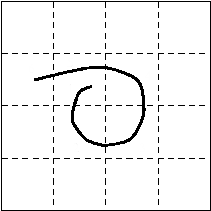
\includegraphics[scale=0.70]{pics/DAS.png}}
        \subfigure{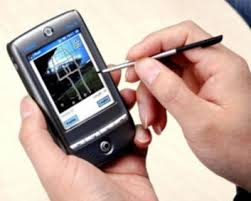
\includegraphics[scale=0.73]{pics/BDAS.jpg}}
        \caption{1) DAS 2)DAS with background}
      \end{figure}

        
    \subsection{Recognition-based}
      Recognition-based passwords are often referred to as cognometric systems \cite{DeAngeli} because the user recall 
      a secret drawing, or sequence of drawings, and the reproduces it as the secret password. Example of implemented 
      recognition-based password schemes are `Passface' and `Deja vu' that uses a sequence of user selected faces/images as a authentication code.

      \begin{figure}[H]
        \centering
        \subfigure{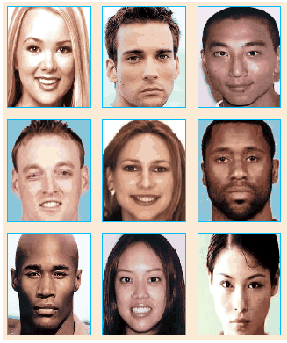
\includegraphics[scale=0.49]{pics/Passface.png}}
        \subfigure{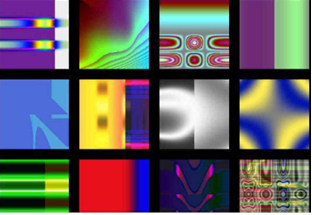
\includegraphics[scale=0.77]{pics/DejaVu.png}}
        \caption{1) Passface 2) Deja vu}
      \end{figure}

    \subsection{Cued-recall}
      Cued-recall are often referred to locimetric systems \cite{DeAngeli}. With cued-recall authentication typically 
      require the users to remember and target a specific location within and image. This is a version of a recall-based 
      authentication, but helps the user with the recall by showing an image and not just an grid or canvas. It is allso 
      different from the recognition-based approah becuase the user need to indentify spesific locations in an image as a whole. 
      One of the known Cued-Recall password scheme are PassPoints.

      \begin{figure}[H]
        \centering
        \subfigure{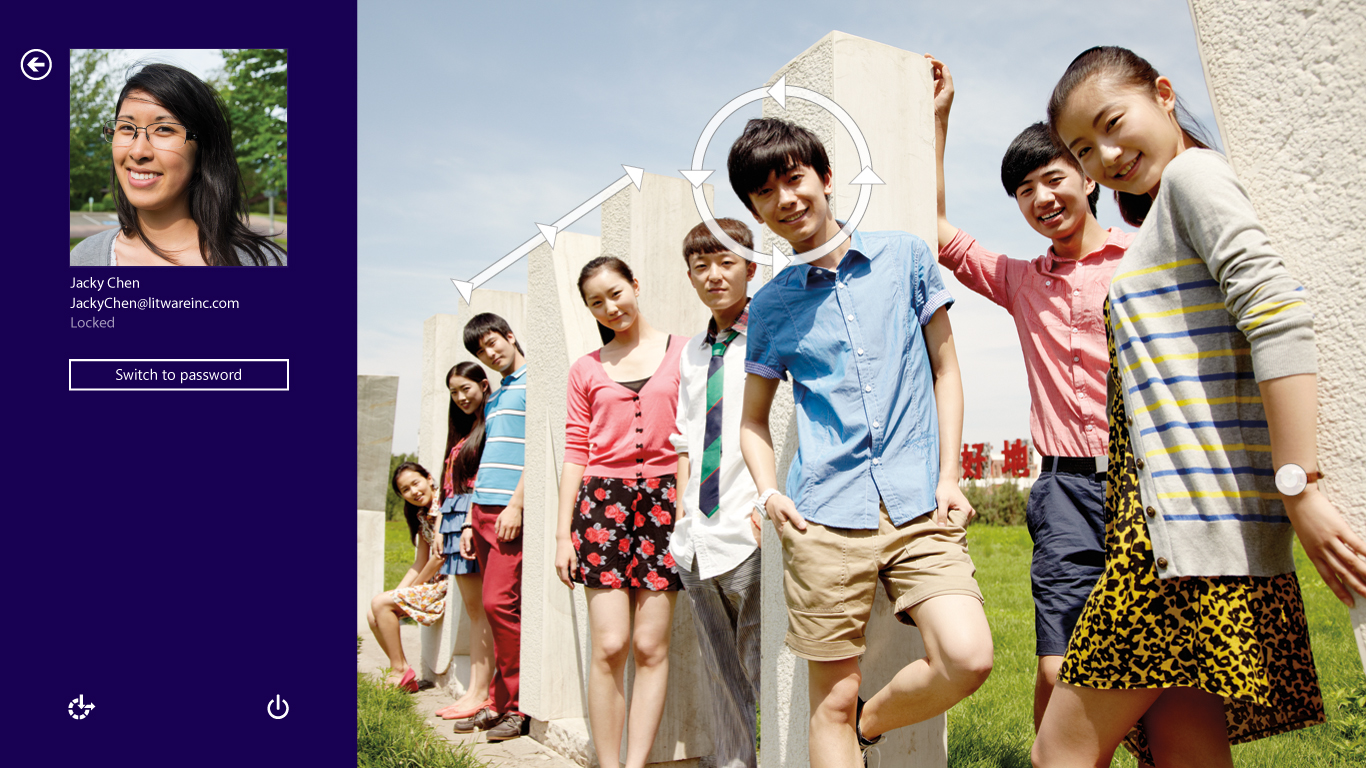
\includegraphics[scale=0.24]{pics/Passpoint.jpg}}
        \caption{1) Passpoints}
      \end{figure}

  \clearpage
  \section{Android Unlock Pattern}

    % When was the first unlock pattern made
    % Hvorfor er dette en standard for bare android og ikke ios?

    There are many different graphical passwors schemes, but the Unlock Pattern is one of the most commonly used screen 
    locks on mobile devices. It was first launched for Android devices, but since it increasingly popularity it have been 
    lauched own apps for using the same unlock patterns on ios.

    The Android password patterns are a special case of the Pass-Go scheme with a restricted grid on 3x3 points. The settings
    on Android phones provides a default setting for using the Unlock pattern. 
    The rules are simple: 
        \begin{itemize}
            \item The pattern needs to have the length 4
            \item You cannot vist the same node twice.
        \end{itemize}

    \begin{figure}[H]
        \centering
        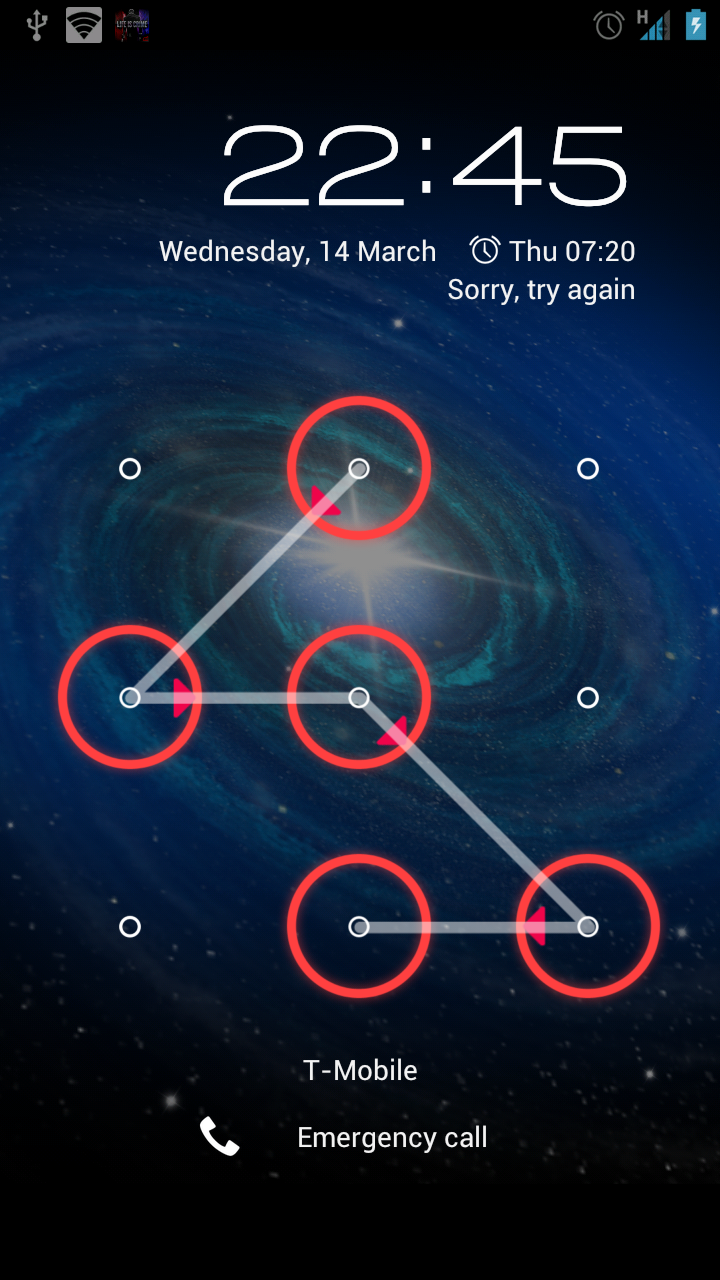
\includegraphics[scale=0.8]{pics/patternLock.png}
    \end{figure}

  \subsection{Passphrase and PIN's vs. graphical passwords}

  \subsection{A password are more then just a password}

    If you take a walk in the street and ask a random person ``what is a password?'', 
    you probably get the aswer ``its letters and digits''. Passwords are so much more than just letter and digits. 

    Nowadays everything we do require you to keep this secret called a password. Your work, you're social life, 
    even you're private life is forcing you to keep track of passwords. How do you keep track of all of them?
    You probably keep the same password at many places. 


 \cite{Uellenbeck} 